\documentclass[conference]{IEEEtran}
\IEEEoverridecommandlockouts

\usepackage{cite}
\usepackage{amsmath,amssymb}
\usepackage{graphicx}
\usepackage{booktabs}
\usepackage{array}
\usepackage{listings}
\usepackage{xcolor}
\usepackage{tikz}
\usetikzlibrary{positioning,arrows.meta,calc}
\usepackage[hidelinks]{hyperref}

\lstdefinestyle{code}{
  basicstyle=\ttfamily\scriptsize,
  columns=fullflexible,
  keepspaces=true,
  breaklines=true,
  frame=tb,
  framesep=3pt,
  aboveskip=6pt,
  belowskip=4pt,
  keywordstyle=\bfseries,
  commentstyle=\itshape\color{black!60},
  showstringspaces=false,
}
\lstdefinelanguage{PGSQL}[]{SQL}{
  morekeywords={RETURNS,LANGUAGE,TRIGGER,EXECUTE,FUNCTION,RECURSIVE,FILTER,COALESCE,NULLIF,
    IF,THEN,ELSIF,END,BEFORE,AFTER,EACH,ROW,DISTINCT,ON,UNNEST,ARRAY,RETURN,NEW,OLD,TG_OP,
    UNION,ALL,WITH,REPLACE,VIEW,IS,FROM,JOIN},
  sensitive=false,
}

\begin{document}

\title{TaskFlow: Database-Enforced Integrity, Auditing\\and Analytics for Project and Task Management}

% TODO: replace the bracketed placeholders with your own details.
\author{\IEEEauthorblockN{Prithvi Raghu}
\IEEEauthorblockA{\textit{[Department of Computer Science and Engineering]} \\
\textit{[Institution Name]}\\
{[City], [Country]} \\
{[institutional e-mail]}}
}

\maketitle

\begin{abstract}
Small productivity applications usually keep their business rules in
application code and treat the database as passive storage. This paper presents
TaskFlow, a project and task management system built on PostgreSQL in which the
database itself carries the rules. The schema has eight relations in third
normal form. It uses six CHECK and six UNIQUE constraints and twelve foreign
keys with explicit \texttt{ON DELETE} actions. Two PL/pgSQL triggers record an
audit trail of task status changes and maintain completion timestamps. Two
views compute project and milestone progress on every read. Thirteen analytical
queries, ranging from simple joins to a recursive common table expression over a
self-referencing many-to-many relationship, run live in a read-only transaction.
Task dependencies form a directed graph whose acyclicity cannot be expressed as a
row-level constraint, so it is enforced by a depth-first search before each
insertion. A test suite of 47 cases runs against a real PostgreSQL instance and
verifies constraints, triggers, views, cascades and transactional rollback. An
independent review found one cycle-detection defect, which led to a stricter
invariant that keeps dependency edges within a single project. The results show
that placing integrity and auditing in the database makes them hold for every
client, including ad-hoc SQL sessions, at negligible cost to application
complexity.
\end{abstract}

\begin{IEEEkeywords}
relational databases, PostgreSQL, integrity constraints, triggers, views,
normalization, recursive queries, transactions, task management
\end{IEEEkeywords}

% ---------------------------------------------------------------------------
\section{Introduction}

Project and task trackers are a standard example of a data-intensive
application. Users own projects, projects are split into milestones and tasks,
tasks are labelled and can depend on one another, and managers want to know how
far along each project is and what is overdue. Most frameworks encourage
developers to implement these rules in the application tier: validation in
forms, cascades in the object-relational mapper (ORM), audit logs in service
code, and progress figures computed in loops. The database then accepts any row
that a different client, a migration script or a person at a \texttt{psql}
prompt cares to write.

TaskFlow takes the opposite position. The relational model~\cite{codd1970}
and its supporting theory of constraints, normal forms and
transactions~\cite{silberschatz2019,elmasri2016} are applied so that the
database guarantees the properties that matter regardless of which client
touches it. The contributions of this work are:
\begin{itemize}
  \item a normalized schema (Section~\ref{sec:design}) whose integrity rules,
        including referential actions, are declared in PostgreSQL rather than
        emulated by the ORM;
  \item an audit and timestamp mechanism implemented with triggers, so the
        history table is written \emph{only} by the database
        (Section~\ref{sec:dbfeatures});
  \item progress reporting through views and a catalogue of thirteen analytical
        queries, including a recursive prerequisite-chain query, exposed
        read-only in the application (Section~\ref{sec:queries});
  \item an analysis of a constraint that a CHECK clause cannot express,
        dependency-graph acyclicity, and of a defect in its first implementation
        (Section~\ref{sec:app});
  \item a test-based evaluation against a live database instance
        (Section~\ref{sec:eval}).
\end{itemize}

% ---------------------------------------------------------------------------
\section{Background and Related Work}

Chen's entity-relationship model~\cite{chen1976} is the usual conceptual
starting point, and Codd's normal forms~\cite{codd1972}, as summarised by
Kent~\cite{kent1983}, guide the logical design. Declarative integrity
constraints and referential actions are part of standard SQL and are covered in
detail in database textbooks~\cite{silberschatz2019,elmasri2016,ramakrishnan2003}.
Active database systems extend the passive model with event-condition-action
rules, i.e. triggers~\cite{widom1996}. PostgreSQL, which descends from the
POSTGRES project~\cite{stonebraker1986}, implements these as row-level PL/pgSQL
triggers~\cite{pgdocs}. Recursive queries entered the standard with
SQL:1999~\cite{sql1999} and allow transitive closure to be computed inside the
engine. Transactions with atomicity, consistency, isolation and durability
(ACID)~\cite{haerder1983,gray1993} ensure that multi-statement updates are
all-or-nothing.

Web frameworks such as Django~\cite{djangodocs} provide an ORM that, by default,
implements \texttt{on\_delete} behaviour in Python and creates foreign keys
without referential actions. TaskFlow uses Django for the user interface and
migrations, but deliberately pushes integrity, cascades, auditing and reporting
down into PostgreSQL.

% ---------------------------------------------------------------------------
\section{System Overview}

TaskFlow is a three-tier web application (Fig.~\ref{fig:arch}). The browser
renders server-side HTML templates, with Chart.js used only to draw dashboard
charts from data embedded by the server. The application tier is Django~5.1 on
Python~3.12, connected to PostgreSQL~16 through psycopg~3. All raw SQL lives in
four files (\texttt{triggers.sql}, \texttt{views.sql}, \texttt{queries.sql} and
\texttt{transactions.sql}). The first two are installed by migrations using
\texttt{RunSQL}, so a fresh clone reaches the full schema with a single
\texttt{migrate} command. Credentials come from an environment file that is
never committed.

Functionally, the system offers registration and login, project, milestone and
task management, categories, tags, task prerequisites with a ``blocked''
indicator, one-click status changes, a status-history timeline, search with
filtering and sorting, CSV export of the filtered list, a dashboard, and an
analytics page. Every query is scoped to the signed-in user, and objects owned
by another user return HTTP~404.

\begin{figure}[t]
\centering
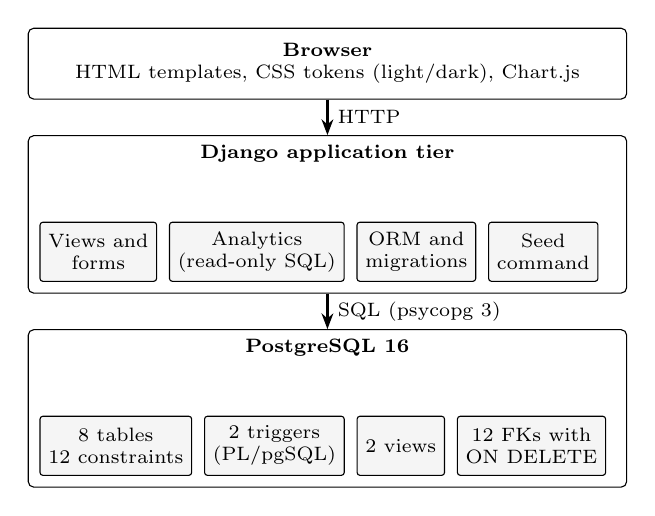
\begin{tikzpicture}[
  font=\scriptsize,
  layer/.style={draw, rounded corners=2pt, minimum width=7.6cm, align=center, inner sep=4pt},
  box/.style={draw, rounded corners=1pt, fill=black!4, align=center, inner sep=3pt, minimum height=0.75cm},
  arr/.style={-{Stealth[length=2mm]}, thick}]
  \node[layer, minimum height=0.9cm] (ui) {\textbf{Browser}\\HTML templates, CSS tokens (light/dark), Chart.js};
  \node[layer, below=0.45cm of ui, minimum height=2.0cm] (app) {};
  \node[anchor=north] at (app.north) {\textbf{Django application tier}};
  \node[box, anchor=south west] (v) at ($(app.south west)+(0.15,0.15)$) {Views and\\forms};
  \node[box, right=0.15cm of v] (a) {Analytics\\(read-only SQL)};
  \node[box, right=0.15cm of a] (o) {ORM and\\migrations};
  \node[box, right=0.15cm of o] (s) {Seed\\command};
  \node[layer, below=0.45cm of app, minimum height=2.0cm] (db) {};
  \node[anchor=north] at (db.north) {\textbf{PostgreSQL 16}};
  \node[box, anchor=south west] (t) at ($(db.south west)+(0.15,0.15)$) {8 tables\\12 constraints};
  \node[box, right=0.15cm of t] (tr) {2 triggers\\(PL/pgSQL)};
  \node[box, right=0.15cm of tr] (vw) {2 views};
  \node[box, right=0.15cm of vw] (fk) {12 FKs with\\ON DELETE};
  \draw[arr] (ui.south) -- node[right]{HTTP} (app.north);
  \draw[arr] (app.south) -- node[right]{SQL (psycopg 3)} (db.north);
\end{tikzpicture}
\caption{Three-tier architecture. Integrity, auditing and progress reporting are
implemented in the database tier.}
\label{fig:arch}
\end{figure}

% ---------------------------------------------------------------------------
\section{Database Design}
\label{sec:design}

\subsection{Conceptual Model}

Fig.~\ref{fig:er} shows the entity-relationship model. Four relationships carry
most of the design:
(i)~\emph{project~1:N~task}, where a task belongs to exactly one project;
(ii)~\emph{task~1:N~task\_history}, the audit trail;
(iii)~\emph{task~M:N~tag}, resolved by the junction relation
\texttt{task\_tag}; and
(iv)~a \emph{recursive M:N} relationship from tasks to tasks, resolved by the
junction relation \texttt{task\_dependency}, in which a task may require several
prerequisites and may itself be a prerequisite of several tasks. Milestones and categories relate to tasks optionally (0..1:N), and each
user owns their projects, categories and tags.

\begin{figure*}[t]
\centering
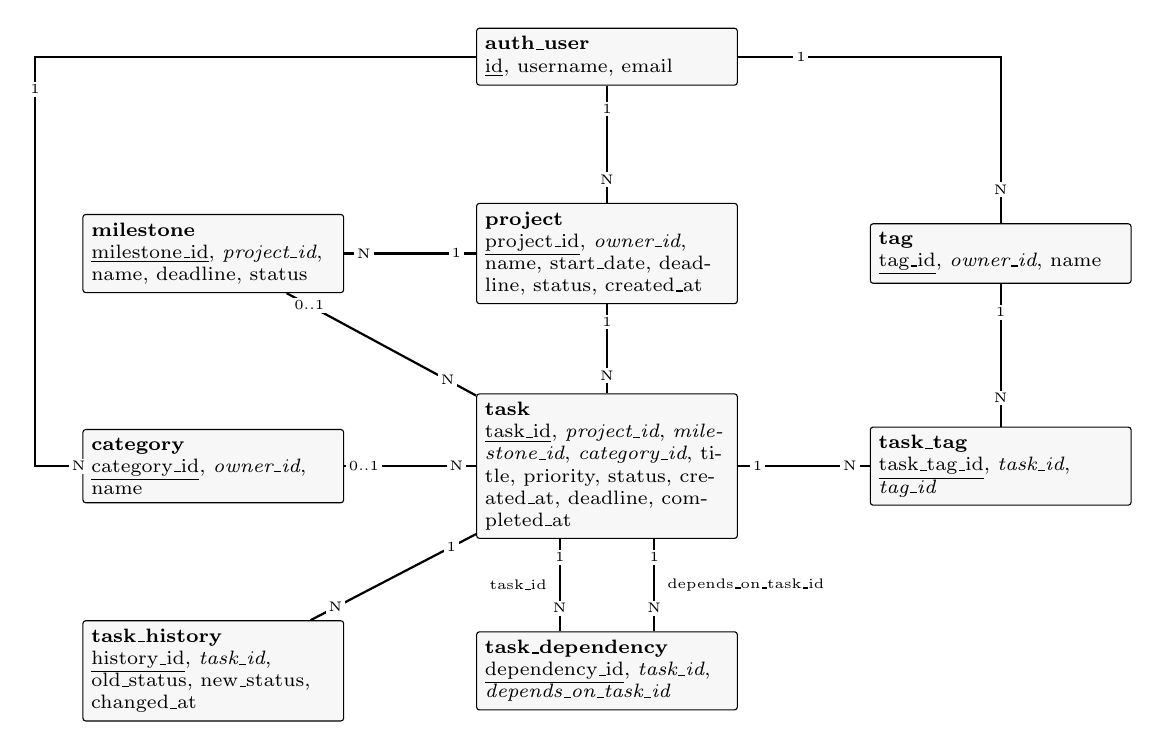
\begin{tikzpicture}[
  font=\scriptsize,
  ent/.style={draw, rounded corners=1pt, align=left, inner sep=3pt, text width=3.1cm, fill=black!3},
  rel/.style={thick},
  card/.style={font=\tiny, fill=white, inner sep=1pt}]
  \node[ent] (user) at (0,1.5)   {\textbf{auth\_user}\\ \underline{id}, username, email};
  \node[ent] (proj) at (0,-1.0)  {\textbf{project}\\ \underline{project\_id}, \textit{owner\_id}, name, start\_date, deadline, status, created\_at};
  \node[ent] (mile) at (-5.0,-1.0) {\textbf{milestone}\\ \underline{milestone\_id}, \textit{project\_id}, name, deadline, status};
  \node[ent] (tagg) at (5.0,-1.0) {\textbf{tag}\\ \underline{tag\_id}, \textit{owner\_id}, name};
  \node[ent] (task) at (0,-3.7)  {\textbf{task}\\ \underline{task\_id}, \textit{project\_id}, \textit{milestone\_id}, \textit{category\_id}, title, priority, status, created\_at, deadline, completed\_at};
  \node[ent] (cat)  at (-5.0,-3.7) {\textbf{category}\\ \underline{category\_id}, \textit{owner\_id}, name};
  \node[ent] (tt)   at (5.0,-3.7) {\textbf{task\_tag}\\ \underline{task\_tag\_id}, \textit{task\_id}, \textit{tag\_id}};
  \node[ent] (hist) at (-5.0,-6.3) {\textbf{task\_history}\\ \underline{history\_id}, \textit{task\_id}, old\_status, new\_status, changed\_at};
  \node[ent] (dep)  at (0,-6.3) {\textbf{task\_dependency}\\ \underline{dependency\_id}, \textit{task\_id}, \textit{depends\_on\_task\_id}};

  \draw[rel] (user) -- node[card,pos=0.2]{1} node[card,pos=0.8]{N} (proj);
  \draw[rel] (user.east) -| node[card,pos=0.12]{1} node[card,pos=0.9]{N} (tagg.north);
  \draw[rel] (user.west) -- ++(-5.6,0) |- node[card,pos=0.04]{1} node[card,pos=0.96]{N} (cat.west);
  \draw[rel] (proj) -- node[card,pos=0.15]{1} node[card,pos=0.85]{N} (mile);
  \draw[rel] (proj) -- node[card,pos=0.2]{1} node[card,pos=0.8]{N} (task);
  \draw[rel] (mile) -- node[card,pos=0.12]{0..1} node[card,pos=0.85]{N} (task);
  \draw[rel] (cat) -- node[card,pos=0.15]{0..1} node[card,pos=0.85]{N} (task);
  \draw[rel] (tagg) -- node[card,pos=0.2]{1} node[card,pos=0.8]{N} (tt);
  \draw[rel] (task) -- node[card,pos=0.15]{1} node[card,pos=0.85]{N} (tt);
  \draw[rel] (task) -- node[card,pos=0.15]{1} node[card,pos=0.85]{N} (hist);
  \draw[rel] ($(task.south)+(-0.6,0)$) -- node[card,pos=0.2]{1} node[card,pos=0.75]{N} node[left=1pt,font=\tiny,pos=0.5]{task\_id} ($(dep.north)+(-0.6,0)$);
  \draw[rel] ($(task.south)+(0.6,0)$) -- node[card,pos=0.2]{1} node[card,pos=0.75]{N} node[right=1pt,font=\tiny,pos=0.5]{depends\_on\_task\_id} ($(dep.north)+(0.6,0)$);
\end{tikzpicture}
\caption{Entity-relationship diagram (primary keys underlined, foreign keys in
italics). \texttt{task\_tag} resolves the task--tag M:N relationship;
\texttt{task\_dependency} resolves the recursive task--task M:N relationship.}
\label{fig:er}
\end{figure*}

\subsection{Relational Schema and Constraints}

Each entity maps to one relation with a surrogate \texttt{bigint} identity key
and an explicit table name, so that raw SQL reads naturally
(\texttt{task.task\_id}). Natural keys are not discarded. They are kept as
UNIQUE constraints, so surrogate keys do not weaken integrity.
Table~\ref{tab:constraints} lists the declared rules.

\begin{table}[t]
\caption{Declared Integrity Constraints}
\label{tab:constraints}
\centering
\scriptsize
\setlength{\tabcolsep}{3pt}
\begin{tabular}{@{}l l p{4.1cm}@{}}
\toprule
\textbf{Relation} & \textbf{Type} & \textbf{Rule} \\
\midrule
category, tag & UNIQUE & (owner\_id, name) \\
project & UNIQUE & (owner\_id, name) \\
project & CHECK & deadline $\geq$ start\_date \\
project & CHECK & status $\in$ \{PLANNED, ACTIVE, COMPLETED, ON\_HOLD\} \\
milestone & UNIQUE & (project\_id, name) \\
milestone & CHECK & status $\in$ \{PENDING, IN\_PROGRESS, COMPLETED\} \\
task & CHECK & priority $\in$ \{LOW, MEDIUM, HIGH\} \\
task & CHECK & status $\in$ \{PENDING, IN\_PROGRESS, BLOCKED, COMPLETED\} \\
task\_tag & UNIQUE & (task\_id, tag\_id) \\
task\_dependency & UNIQUE & (task\_id, depends\_on\_task\_id) \\
task\_dependency & CHECK & task\_id $\neq$ depends\_on\_task\_id \\
\midrule
milestone, task, task\_tag, & FK & ON DELETE CASCADE from parent \\
\quad task\_dependency, task\_history & & \\
task.milestone\_id, & FK & ON DELETE SET NULL \\
\quad task.category\_id & & \\
project, category, tag & FK & owner\_id ON DELETE CASCADE \\
\bottomrule
\end{tabular}
\end{table}

By default, Django emulates referential actions in Python and creates foreign keys
without them, so a \texttt{DELETE} issued outside the application would either
fail or leave orphans. TaskFlow adds a small migration helper that replaces each
generated key with a named one carrying the intended action. As a result,
deleting a project in \texttt{psql} removes its milestones, tasks, history and
link rows. Deleting a milestone keeps its tasks but clears their
\texttt{milestone\_id}. The helper runs in a migration separate from the one
that creates the table, because Django defers foreign-key creation to the end of
each migration.

\subsection{Normalization}

The design was derived from a single unnormalised ``task sheet'' holding owner,
project, milestone and task attributes plus three multi-valued columns (tags,
prerequisites and a status log). Table~\ref{tab:nf} summarises the
decomposition. In 1NF the repeating groups move into their own relations keyed
by the task's identifying attributes (owner, project, title). In 2NF, the partial
dependencies $\textit{owner}\rightarrow\textit{email}$ and
$(\textit{owner},\textit{project})\rightarrow\textit{project attributes}$
produce \texttt{user} and \texttt{project}. In 3NF, the transitive dependency
$\textit{task key}\rightarrow\textit{milestone}\rightarrow\textit{milestone
deadline, status}$ produces \texttt{milestone}. Every remaining determinant is
a candidate key, so the final schema is also in Boyce--Codd normal form.

\begin{table}[t]
\caption{Normalization Steps}
\label{tab:nf}
\centering
\scriptsize
\setlength{\tabcolsep}{3pt}
\begin{tabular}{@{}l p{2.9cm} p{3.3cm}@{}}
\toprule
\textbf{Form} & \textbf{Problem removed} & \textbf{Relations produced} \\
\midrule
UNF $\rightarrow$ 1NF & lists in tags, prerequisites, status log & task, task\_tag, task\_dependency, task\_history \\
1NF $\rightarrow$ 2NF & partial dependencies on the composite key & user, project, tag, category \\
2NF $\rightarrow$ 3NF & milestone attributes transitively dependent on the task key & milestone \\
3NF $\rightarrow$ tables & wide natural keys & surrogate keys plus UNIQUE natural keys \\
\bottomrule
\end{tabular}
\end{table}

Two apparent redundancies are deliberate. \texttt{task.completed\_at} could be
derived from \texttt{task\_history}, but it is stored so that duration queries
avoid scanning the history, and a trigger keeps it consistent. The progress
figures look like stored totals but are views, recomputed on every read, so
they cannot drift.

% ---------------------------------------------------------------------------
\section{Database-Level Features}
\label{sec:dbfeatures}

\subsection{Triggers}

\texttt{trg\_task\_status\_history} is an \texttt{AFTER INSERT OR UPDATE OF
status} row trigger. On insert it records $(\texttt{NULL}\rightarrow s)$. On
update it records $(s_{old}\rightarrow s_{new})$ only when the two differ, which
it tests with \texttt{IS DISTINCT FROM} so that no-op updates leave no trace
(Listing~\ref{lst:trigger}). It uses \texttt{clock\_timestamp()} rather than
\texttt{now()}, so several changes made in one transaction still receive
distinct, ordered times. The application never inserts into
\texttt{task\_history}, so the audit trail covers every client.

\begin{lstlisting}[style=code,float=tb,language=PGSQL,caption={Status-history trigger function},label={lst:trigger}]
CREATE OR REPLACE FUNCTION fn_task_status_history()
RETURNS trigger LANGUAGE plpgsql AS $$
BEGIN
  IF TG_OP = 'INSERT' THEN
    INSERT INTO task_history (task_id, old_status, new_status, changed_at)
    VALUES (NEW.task_id, NULL, NEW.status, clock_timestamp());
  ELSIF OLD.status IS DISTINCT FROM NEW.status THEN
    INSERT INTO task_history (task_id, old_status, new_status, changed_at)
    VALUES (NEW.task_id, OLD.status, NEW.status, clock_timestamp());
  END IF;
  RETURN NULL;
END; $$;
\end{lstlisting}

\texttt{trg\_task\_completed\_at} is a \texttt{BEFORE INSERT OR UPDATE} trigger
that keeps \texttt{completed\_at} consistent with \texttt{status}. The field is
stamped when a task becomes COMPLETED, cleared when it leaves that state, and
otherwise preserved. Preservation matters because an ORM save that rewrites
every column would otherwise overwrite the stored timestamp with a stale value.

\subsection{Views}

\texttt{v\_project\_progress} aggregates each project's tasks with a
\texttt{LEFT JOIN}, so projects without tasks still appear. It uses
\texttt{COUNT(\ldots) FILTER (WHERE \ldots)} for completed and overdue counts,
and \texttt{NULLIF} to avoid division by zero in the completion percentage.
\texttt{v\_milestone\_progress} does the same per milestone. Both are mapped to
read-only (\emph{unmanaged}) ORM models, which lets the dashboard and project
pages join to them without the application recomputing any figure.

\subsection{Transactions}

Creating a project together with its initial milestones runs inside a single
transaction in the application, so a failure on any milestone insert also undoes
the project. A companion SQL script demonstrates both outcomes in
\texttt{psql}. The first block commits a project, two milestones and a task
together. The second inserts a project and two milestones, then attempts a task
with priority \texttt{'URGENT'}. That insert violates \texttt{ck\_task\_priority},
the transaction enters the aborted state and refuses further statements, and
after \texttt{ROLLBACK} the project and milestone counts are both zero, as
atomicity requires~\cite{haerder1983}.

% ---------------------------------------------------------------------------
\section{Application-Layer Rules}
\label{sec:app}

\subsection{Acyclic Task Dependencies}

The prerequisite relation must form a directed acyclic graph, otherwise some
tasks could never be completed. A CHECK constraint sees only one row, so it can
reject the trivial cycle $t \rightarrow t$ but not
$a \rightarrow b \rightarrow c \rightarrow a$, which spans several rows.
Before inserting an edge $t \rightarrow p$, the dependency form therefore runs an
iterative depth-first search~\cite{tarjan1972} from $p$ over the existing
edges. If $t$ is reachable, the new edge would close a cycle, and the form
reports the full path, e.g.\ ``A $\rightarrow$ C $\rightarrow$ B $\rightarrow$
A'' (Listing~\ref{lst:dfs}). The search is $O(V+E)$ in the user's dependency
graph.

\begin{lstlisting}[style=code,float=tb,language=Python,caption={Reachability check used before inserting a dependency edge},label={lst:dfs}]
def find_dependency_path(start_id, target_id, edges):
    stack, seen = [(start_id, [start_id])], set()
    while stack:
        node, path = stack.pop()
        if node == target_id:
            return path   # edge would close a cycle
        if node in seen:
            continue
        seen.add(node)
        for nxt in edges.get(node, ()):
            stack.append((nxt, path + [nxt]))
    return None
\end{lstlisting}

The first implementation loaded only the edges of the task's current project.
An independent review showed that a task could be moved to another project
while keeping its links. That left edges crossing projects, which the
per-project search could not see, and a three-task cycle could then be
inserted. The fix has two parts. The search now loads every edge owned by the
user, and a task that has prerequisites or dependents can no longer change
project. This keeps an invariant that every dependency edge lies within one
project. The case shows that application-level checks need the same scrutiny
as declarative constraints, because they protect only the invariants they can
see. A database trigger running the recursive query of Section~\ref{sec:queries}
would close the remaining gap for clients other than the web application.

\subsection{Other Rules}

Completing a task with open prerequisites is refused by both the edit form and
the quick-status endpoint. A task's milestone must belong to its project, and
its deadline cannot precede the project's start. Every query is filtered by
owner, and form choice sets are restricted to the user's rows, so a forged
identifier fails validation rather than leaking data. Filter values outside the
allowed set produce an explicit error and an empty result instead of silently
being ignored. CSV export prefixes cells that start with \texttt{=}, \texttt{+},
\texttt{-} or \texttt{@}, which neutralises spreadsheet formula injection.

% ---------------------------------------------------------------------------
\section{Analytical Queries}
\label{sec:queries}

Table~\ref{tab:queries} lists the thirteen analytical queries and the concepts
each demonstrates. The queries live in a single SQL file, which can be run
directly in \texttt{psql} using variables \texttt{:owner\_id} and
\texttt{:task\_id}. The analytics page parses the same file, converts those
variables into bound parameters and executes every query in a
\texttt{READ ONLY} transaction with a five-second statement timeout. The SQL
shown on screen is therefore exactly the SQL that ran, and user input never
becomes part of the query text.

\begin{table}[t]
\caption{Analytical Queries and Concepts}
\label{tab:queries}
\centering
\scriptsize
\setlength{\tabcolsep}{3pt}
\begin{tabular}{@{}r p{3.6cm} p{3.2cm}@{}}
\toprule
\textbf{\#} & \textbf{Question answered} & \textbf{Concepts} \\
\midrule
1 & Total and completed tasks per project & LEFT JOIN, GROUP BY, FILTER \\
2 & Completion percentage and stage & CASE, aggregates, NULLIF \\
3 & Overdue incomplete tasks & date filtering and arithmetic \\
4 & Tasks by status and priority & two-column GROUP BY \\
5 & Top five categories by task count & ORDER BY, LIMIT \\
6 & Milestone completion & querying a view \\
7 & Projects with $>$5 open tasks & WHERE vs.\ HAVING \\
8 & Status history of a task & trigger-written rows \\
9 & Tasks blocked by open prerequisites & EXISTS, correlated subquery \\
10 & Project(s) with most overdue tasks & nested subquery, ties kept \\
11 & Average days to complete & interval arithmetic, ROLLUP \\
12 & Projects above average completion & scalar subquery \\
13 & Full prerequisite chain of a task & WITH RECURSIVE, cycle guard \\
\bottomrule
\end{tabular}
\end{table}

Query~10 compares each project's count with the maximum of a derived table in
a \texttt{HAVING} clause, instead of using \texttt{ORDER BY \ldots{} LIMIT 1}.
On the demonstration data two projects tie with three overdue tasks, and
\texttt{LIMIT 1} would arbitrarily hide one of them. Query~13 computes the
transitive closure of the prerequisite relation (Listing~\ref{lst:cte}). The
recursive member carries the visited path as an array and stops when it would
revisit a node, so even corrupted data cannot make it loop.
\texttt{DISTINCT ON} keeps the shortest path to each ancestor.
Table~\ref{tab:chain} shows its output for one task.

\begin{lstlisting}[style=code,float=tb,language=PGSQL,caption={Recursive prerequisite chain (Q13, abridged)},label={lst:cte}]
WITH RECURSIVE chain AS (
  SELECT d.depends_on_task_id AS task_id, 1 AS depth,
         ARRAY[d.task_id, d.depends_on_task_id] AS path
  FROM task_dependency d WHERE d.task_id = :task_id
  UNION ALL
  SELECT d.depends_on_task_id, c.depth + 1,
         c.path || d.depends_on_task_id
  FROM chain c
  JOIN task_dependency d ON d.task_id = c.task_id
  WHERE d.depends_on_task_id <> ALL (c.path)  -- cycle guard
)
SELECT DISTINCT ON (c.task_id) c.depth, t.title, t.status
FROM chain c JOIN task t ON t.task_id = c.task_id
ORDER BY c.task_id, c.depth;
\end{lstlisting}

\begin{table}[t]
\caption{Q13 Output for ``Colour and Type Tokens''}
\label{tab:chain}
\centering
\scriptsize
\begin{tabular}{@{}c l l@{}}
\toprule
\textbf{Depth} & \textbf{Prerequisite} & \textbf{Status} \\
\midrule
1 & Choose headless CMS & COMPLETED \\
2 & Draft sitemap & COMPLETED \\
2 & Low-fidelity wireframes & COMPLETED \\
3 & Audit current site analytics & COMPLETED \\
4 & Stakeholder interviews & COMPLETED \\
\bottomrule
\end{tabular}
\end{table}

% ---------------------------------------------------------------------------
\section{Evaluation}
\label{sec:eval}

\subsection{Demonstration Data}

A seeding command generates reproducible data from a fixed random seed, with
dates relative to the current day so that some tasks are always overdue. It
creates 2 users, 4 projects, 12 milestones and 60 tasks (25 completed, 12 in
progress, 8 blocked and 15 pending), along with 29 dependency edges and 50
task--tag links. Tasks are inserted as PENDING and moved through their statuses
with ordinary \texttt{UPDATE}s, so the trigger writes all 148 history rows. The
trigger-written timestamps are then spread over each task's lifetime, so the
timeline and duration figures are realistic. For the primary user, the views
report 21 of 45 tasks completed (46.7\%). Query~2 classifies the three projects
at 60.0\%, 53.3\% and 26.7\%, and Query~11 gives a mean of 16.9 days from
creation to completion. Two independent runs of the seed command produced
byte-identical content hashes over tasks, tags, dependencies and history.

\subsection{Automated Tests}

The test suite runs against a real PostgreSQL test database built by the same
migrations, including the raw-SQL triggers and views. No in-memory substitute is
used, so constraints and triggers are exercised as deployed.
Table~\ref{tab:tests} groups the 47 cases. Constraint tests insert violating rows
through both the ORM and raw SQL and assert on the named constraint in the error.
The foreign-key test switches to \texttt{SET CONSTRAINTS ALL IMMEDIATE},
because the generated keys are deferrable. The view tests compare the view's
counts with an independent count computed in Python. All 47 tests pass in about
24~s.

\begin{table}[t]
\caption{Test Suite Composition}
\label{tab:tests}
\centering
\scriptsize
\setlength{\tabcolsep}{3pt}
\begin{tabular}{@{}l c p{4.2cm}@{}}
\toprule
\textbf{Group} & \textbf{Tests} & \textbf{Examples} \\
\midrule
CHECK/UNIQUE & 7 & bad priority, status, deadline; duplicate names \\
Foreign keys & 4 & bad FK; raw-SQL cascade and SET NULL; user delete \\
Dependencies (DB) & 2 & self-loop and duplicate edge rejected \\
Triggers & 6 & history on insert/change only; completed\_at set, kept, cleared \\
Transactions & 2 & rollback leaves no rows; commit keeps all \\
Views & 4 & figures equal a manual count; empty project is 0 \\
Cycle detection & 6 & self, 3-cycle, cross-project edges, moves \\
Ownership/status & 3 & login required; other users' rows 404 \\
Atomic creation & 2 & milestone failure rolls back project \\
Analytics & 4 & 13 queries run, scoped per user, recursion \\
Filters/export & 5 & invalid values rejected; CSV honours filters \\
Seed data & 2 & reproducible; history chronological \\
\midrule
\textbf{Total} & \textbf{47} & \\
\bottomrule
\end{tabular}
\end{table}

\subsection{Independent Review}

A separate end-to-end review was carried out on a fresh clone with an empty
database. It ran the Django system checks, a migration-drift check, the full
suite, both SQL scripts, an HTTP smoke test of 21 pages, cross-user access
checks on 12 object URLs, and a query-count check for N+1 patterns (7 queries
for the task list, 21 for the analytics page). It found no injection,
cross-site request forgery or object-reference vulnerabilities, and it reported
four defects: the cross-project cycle described in
Section~\ref{sec:app}, owner foreign keys without database-level cascade,
artificial seed timestamps, and silently ignored invalid filter values. All
four were fixed, each with a regression test that failed before the fix.

% ---------------------------------------------------------------------------
\section{Limitations and Future Work}

Dependency acyclicity is enforced by the application, not the database. A
constraint trigger that runs the recursive query on each insertion into
\texttt{task\_dependency} would extend the guarantee to every client. Date
consistency across levels, such as milestone deadlines lying within the project
period, is not yet checked. The evaluation uses a small dataset. Indexes exist
on every foreign key and on \texttt{(task\_id, changed\_at)}, but behaviour at
larger scale, and the value of partial indexes on open tasks, has not been
measured. Finally, the dashboard loads its charting library from a content
delivery network, so offline deployments would need a local copy.

% ---------------------------------------------------------------------------
\section{Conclusion}

TaskFlow shows that a modest web application can rely on its relational
database for integrity, auditability and reporting rather than reimplementing
them in application code. Declarative constraints and referential actions keep
data valid under any client. Triggers produce an audit trail that the
application cannot bypass, views remove a whole class of stale-total bugs, and
recursive SQL answers graph questions inside the engine. Testing against the
real database engine, together with an independent review, exposed the one
place where an application-level invariant was weaker than intended, and the
stricter single-project invariant now closes that gap.

% ---------------------------------------------------------------------------
\begin{thebibliography}{00}
\bibitem{codd1970} E.~F. Codd, ``A relational model of data for large shared data banks,'' \textit{Commun. ACM}, vol.~13, no.~6, pp.~377--387, Jun. 1970.
\bibitem{chen1976} P.~P.-S. Chen, ``The entity-relationship model---Toward a unified view of data,'' \textit{ACM Trans. Database Syst.}, vol.~1, no.~1, pp.~9--36, Mar. 1976.
\bibitem{codd1972} E.~F. Codd, ``Further normalization of the data base relational model,'' in \textit{Data Base Systems}, R.~Rustin, Ed. Englewood Cliffs, NJ, USA: Prentice-Hall, 1972, pp.~33--64.
\bibitem{kent1983} W.~Kent, ``A simple guide to five normal forms in relational database theory,'' \textit{Commun. ACM}, vol.~26, no.~2, pp.~120--125, Feb. 1983.
\bibitem{silberschatz2019} A.~Silberschatz, H.~F. Korth, and S.~Sudarshan, \textit{Database System Concepts}, 7th~ed. New York, NY, USA: McGraw-Hill, 2019.
\bibitem{elmasri2016} R.~Elmasri and S.~B. Navathe, \textit{Fundamentals of Database Systems}, 7th~ed. Boston, MA, USA: Pearson, 2016.
\bibitem{ramakrishnan2003} R.~Ramakrishnan and J.~Gehrke, \textit{Database Management Systems}, 3rd~ed. New York, NY, USA: McGraw-Hill, 2003.
\bibitem{widom1996} J.~Widom and S.~Ceri, Eds., \textit{Active Database Systems: Triggers and Rules for Advanced Database Processing}. San Francisco, CA, USA: Morgan Kaufmann, 1996.
\bibitem{stonebraker1986} M.~Stonebraker and L.~A. Rowe, ``The design of POSTGRES,'' in \textit{Proc. ACM SIGMOD Int. Conf. Management of Data}, 1986, pp.~340--355.
\bibitem{pgdocs} The PostgreSQL Global Development Group, ``PostgreSQL 16 documentation,'' 2023. [Online]. Available: \url{https://www.postgresql.org/docs/16/}
\bibitem{sql1999} \textit{Information Technology---Database Languages---SQL---Part 2: Foundation (SQL/Foundation)}, ISO/IEC 9075-2:1999, 1999.
\bibitem{haerder1983} T.~Haerder and A.~Reuter, ``Principles of transaction-oriented database recovery,'' \textit{ACM Comput. Surv.}, vol.~15, no.~4, pp.~287--317, Dec. 1983.
\bibitem{gray1993} J.~Gray and A.~Reuter, \textit{Transaction Processing: Concepts and Techniques}. San Mateo, CA, USA: Morgan Kaufmann, 1993.
\bibitem{tarjan1972} R.~Tarjan, ``Depth-first search and linear graph algorithms,'' \textit{SIAM J. Comput.}, vol.~1, no.~2, pp.~146--160, 1972.
\bibitem{djangodocs} Django Software Foundation, ``Django 5.1 documentation,'' 2024. [Online]. Available: \url{https://docs.djangoproject.com/en/5.1/}
\end{thebibliography}

\end{document}
